\subsection{Zooming in} add the results of the maps where duration, velocity, touches and jerk are resolved in xy.

\begin{figure}[h]
\centering
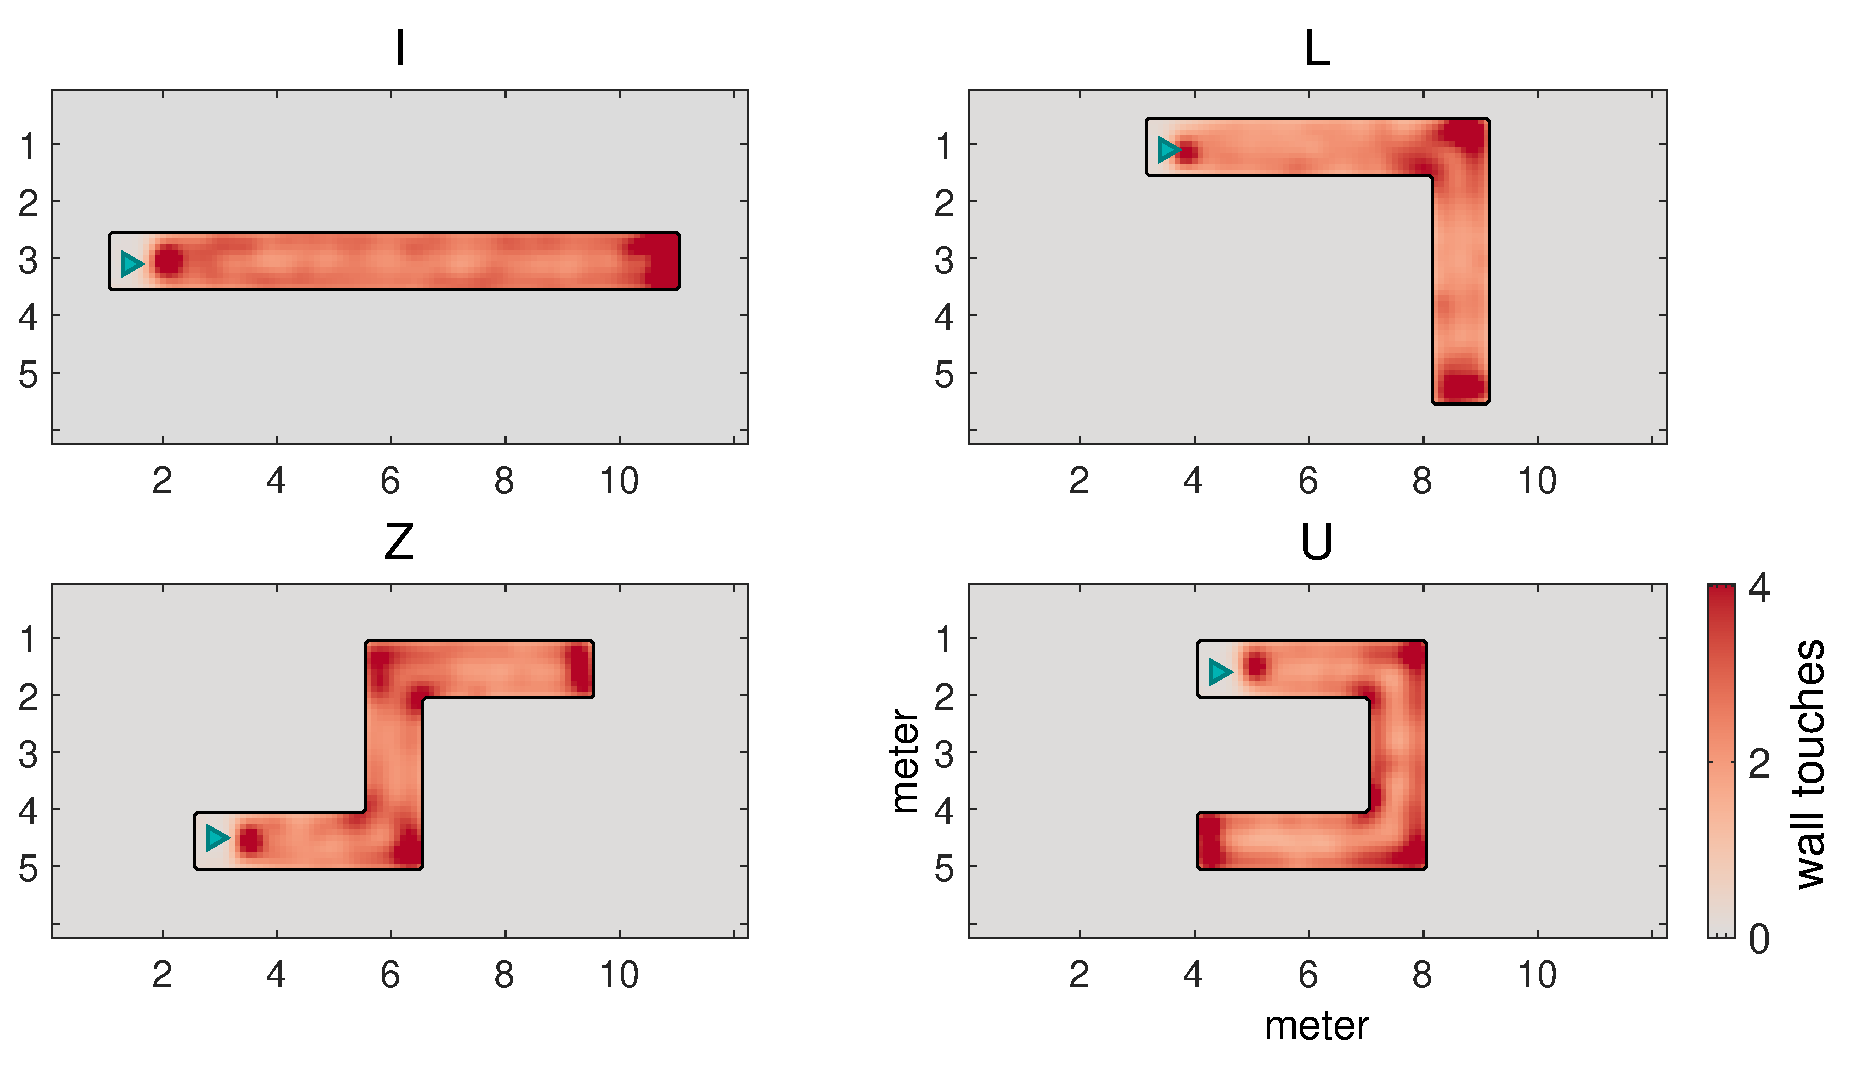
\includegraphics[width=\linewidth]{figures/duration_mean.eps}
\vspace{0pt}
\caption{results duration mean}
\label{results_dur_mean}
\end{figure}

\begin{figure}[h]
\centering
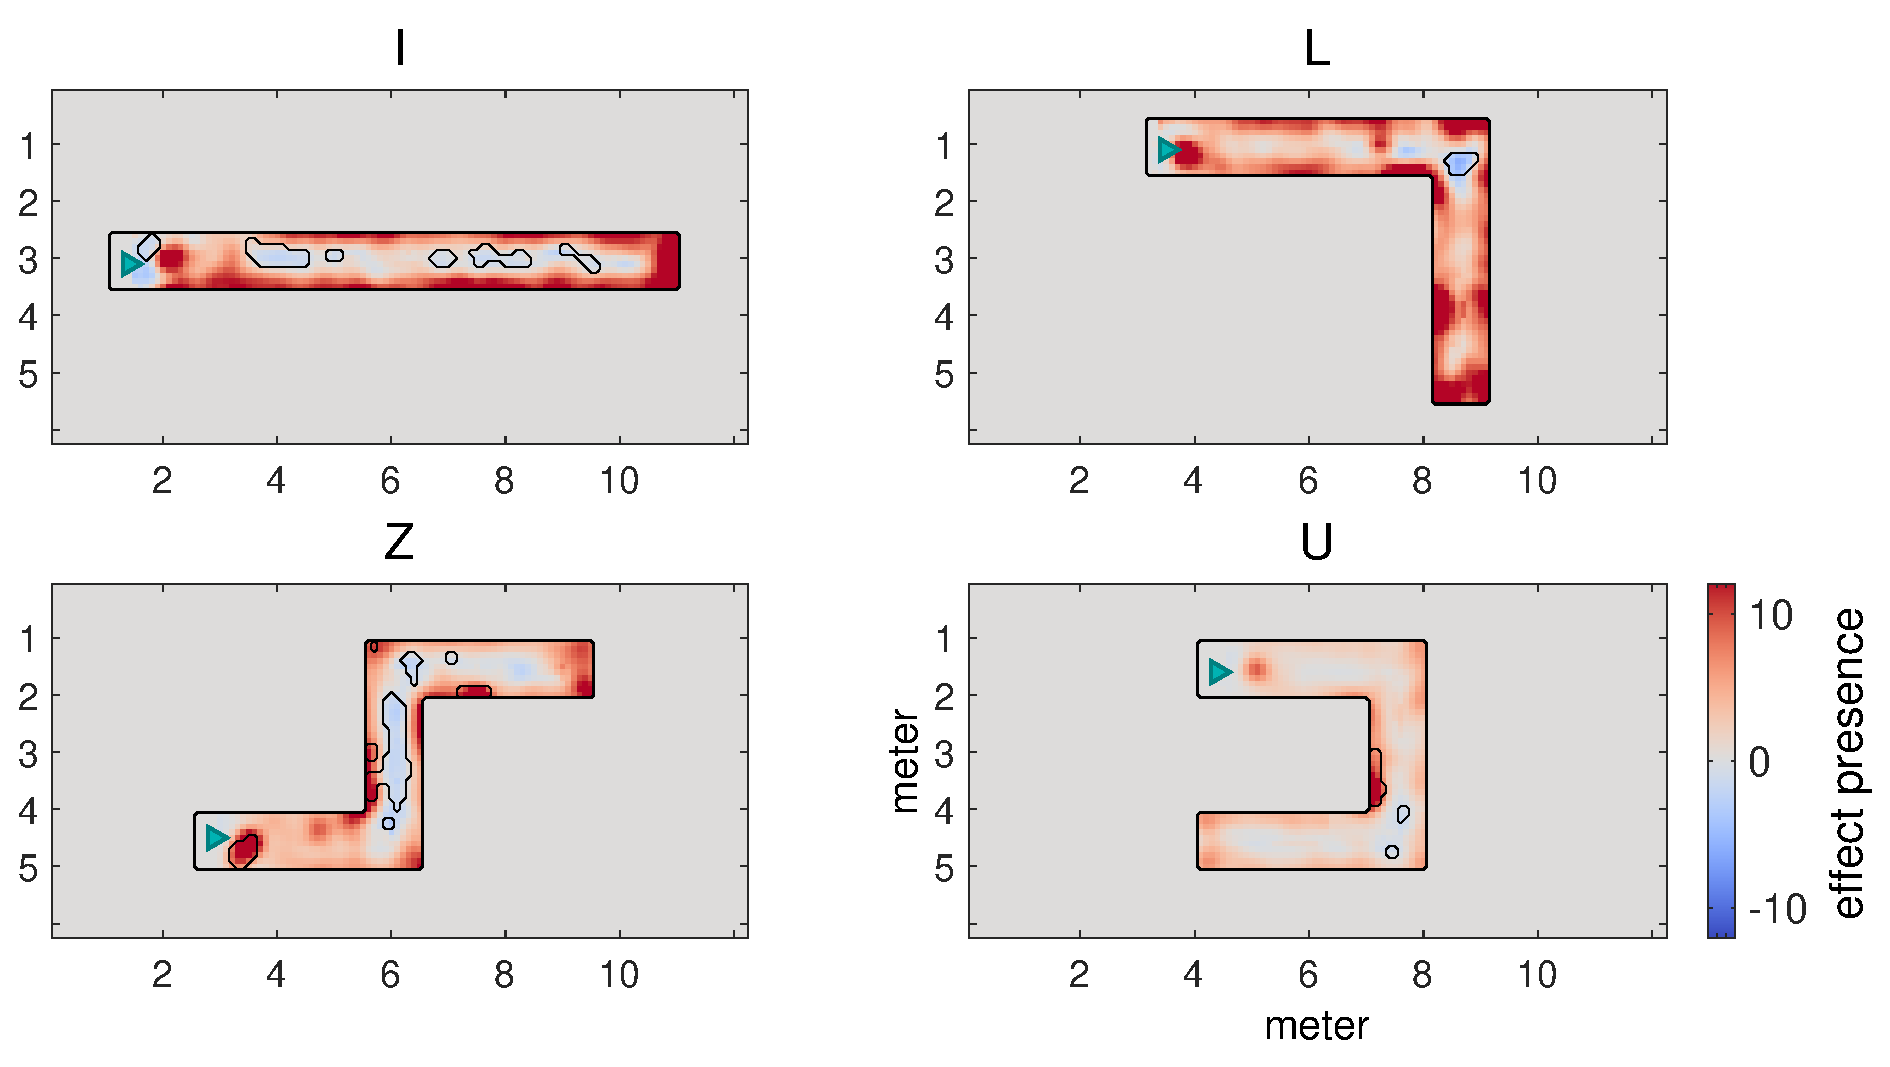
\includegraphics[width=\linewidth]{figures/effect_presence_duration.eps}
\vspace{0pt}
\caption{results duration and velocity}
\label{results_dur_effect}
\end{figure}

\begin{figure}[h]
\centering
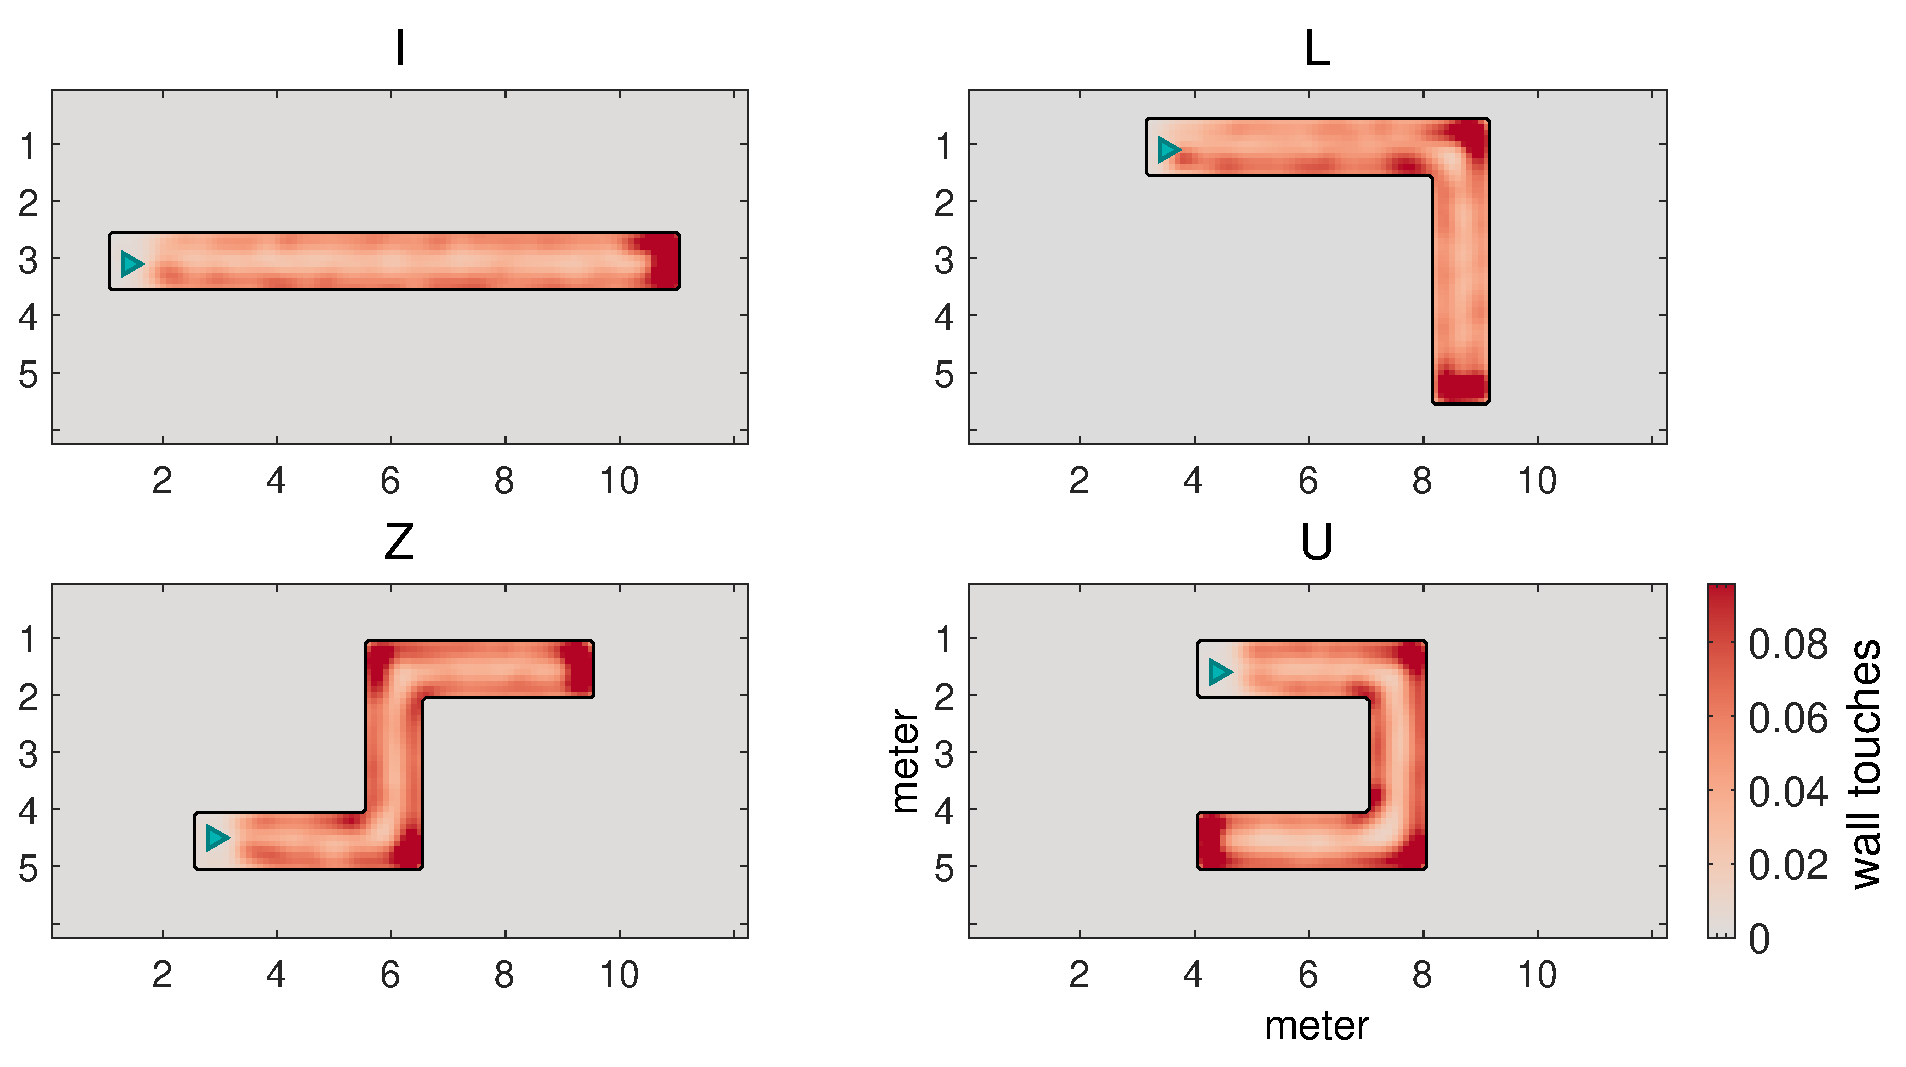
\includegraphics[width=\linewidth]{figures/wall_touches_mean.eps}
\vspace{0pt}
\caption{results duration and velocity}
\label{results_touches_mean}
\end{figure}

\begin{figure}[h]
\centering
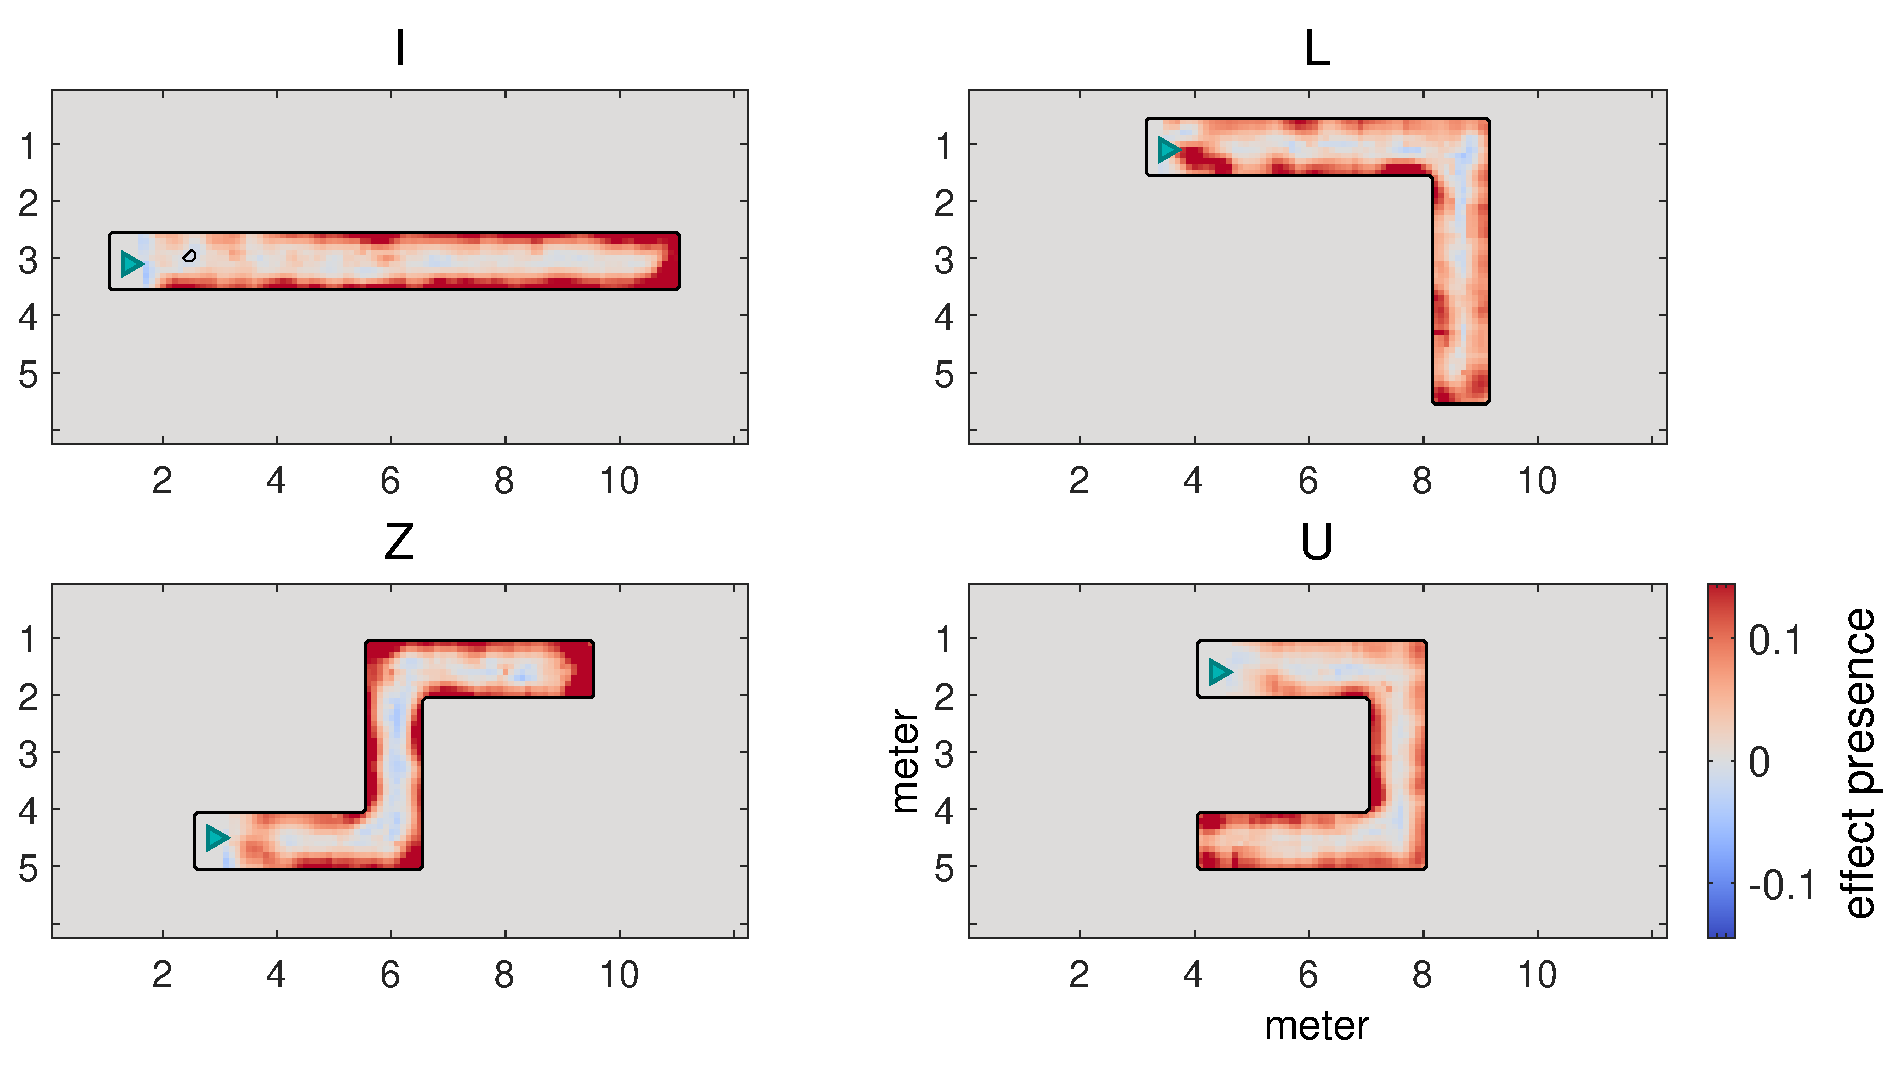
\includegraphics[width=\linewidth]{figures/effect_presence_wall_touches.eps}
\vspace{0pt}
\caption{results duration and velocity}
\label{results_touches_effect}
\end{figure}

\begin{comment}

interpretation histogram binning:
how many samples fall within 1 bin -> samples/srate = duration in seconds per bin, also must consider step size when calculating

what does imagesc return after that? interpretation should stay the same and be sensible -> returns just the gaussian smoothing over the peak that is the histogram count

interpreting regression:
with an increase in presence x more seconds where spent at point xy
for easy interpretation we introduce the reasoning: participants with a higher reported presence spent 1.8 seconds longer at point (4,5 located in the outer corner of the first turn)

interpreting regression:
with an increase in presence participants moved slower closer to the wall and faster in when in the center of the maze path.

for easy interpretation we introduce the reasoning: for each 1 point increase in reported presence, participants walked x km per hour faster when at the center of the maze path and x kmh slower when getting closer to the walls.

\end{comment}